\chapter{Diseño e Implementación} % Main chapter title

\label{Chapter3} % Change X to a consecutive number; for referencing this chapter elsewhere, use \ref{ChapterX}
\definecolor{mygreen}{rgb}{0,0.6,0}
\definecolor{mygray}{rgb}{0.5,0.5,0.5}
\definecolor{mymauve}{rgb}{0.58,0,0.82}

\lstset{ %
  backgroundcolor=\color{white},   % choose the background color; you must add \usepackage{color} or \usepackage{xcolor}
  basicstyle=\footnotesize,        % the size of the fonts that are used for the code
  breakatwhitespace=false,         % sets if automatic breaks should only happen at whitespace
  breaklines=true,                 % sets automatic line breaking
  captionpos=b,                    % sets the caption-position to bottom
  commentstyle=\color{mygreen},    % comment style
  deletekeywords={...},            % if you want to delete keywords from the given language
  %escapeinside={\%*}{*)},          % if you want to add LaTeX within your code
  %extendedchars=true,              % lets you use non-ASCII characters; for 8-bits encodings only, does not work with UTF-8
  %frame=single,	                   % adds a frame around the code
  keepspaces=true,                 % keeps spaces in text, useful for keeping indentation of code (possibly needs columns=flexible)
  keywordstyle=\color{blue},       % keyword style
  language=[ANSI]C,					% the language of the code
  %otherkeywords={*,...},           % if you want to add more keywords to the set
  numbers=left,                    % where to put the line-numbers; possible values are (none, left, right)
  numbersep=5pt,                   % how far the line-numbers are from the code
  numberstyle=\tiny\color{mygray}, % the style that is used for the line-numbers
  rulecolor=\color{black},         % if not set, the frame-color may be changed on line-breaks within not-black text (e.g. comments (green here))
  showspaces=false,                % show spaces everywhere adding particular underscores; it overrides 'showstringspaces'
  showstringspaces=false,          % underline spaces within strings only
  showtabs=false,                  % show tabs within strings adding particular underscores
  stepnumber=1,                    % the step between two line-numbers. If it's 1, each line will be numbered
  stringstyle=\color{mymauve},     % string literal style
  tabsize=2,	                   % sets default tabsize to 2 spaces
  title=\lstname,                   % show the filename of files included with \lstinputlisting; also try caption instead of title
  morecomment=[s]{/*}{*/}%
}

% -------------------------------------

En este capítulo se centra en el proceso de desarrollo del dispositivo, tanto el firmware como hardware, a partir del modelo de desarrollo aplicado.
% --------------------------------------


\section{Implementación del sistema}

\subsection{Resumen del sistema}

El equipo digitaliza señales analógicas provenientes de dos sensores de presión intrarterial del tipo strain-gauge y almacena las señales por períodos de alrededor de 24 hs. Estas señales adquiridas se guardan en una memoria de tipo flash (memoria micro SD), y pueden descargarse a una PC a través de una interfaz USB. Desde la PC se accede a los archivos guardados como un medio de almacenamiento masivo, y se pueden visualizar en cualquier software que permita procesar un archivo de tipo ".csv".

Previo a cada experiencia, el operador configura el equipo desde una terminal Bluetooth, como una tablet o una PC, a través de un protocolo de comunicación muy sencillo que se desarrolló para este dispositivo. A través de esta interfaz se configuran parámetros como la frecuencia de muestreo, la cantidad de canales a usar, ganancia del amplificador programable, seteo de hora y fecha, y finalmente se da inicio a la medición. 

El equipo consiste en un sistema embebido portátil basado en un microcontrolador ARM de 32 bits, Cortex M3: LPC1769, un conversor analógico digital de alta resolución (ADS1292), módulos de comunicación (serie, BLE, USB), almacenamiento masivo (microSD) y módulo de regulación de energía y carga de batería. Puede verse un diagrama en bloques en la Figura \ref{fig:diag_bloques} . Para este proyecto se utilizaron en forma intensiva la gran mayoría de los contenidos y herramientas vistas durante el Carrera de Especialización en Sistemas Embebidos (CESE). Se utilizaron técnicas de Gestión de Proyectos, documentación manual y automática del trabajo, sistema de versionado de software y hardware. En cuanto a lo técnico se emplearon conocimientos específicos sobre arquitectura del microcontrolador, modelos de programación, sistema operativo de tiempo real freeRTOS, protocolos de comunicación (BLE, SPI, USB, y de alto nivel), testing unitarios, etc.


\begin{figure}[!htbp]
	\centering
	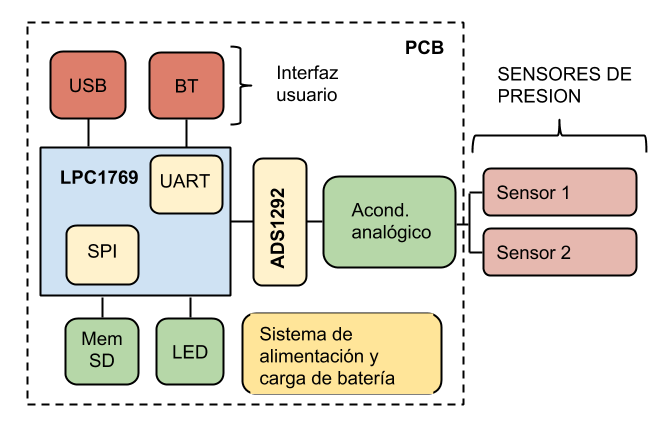
\includegraphics[width=\textwidth]{./Figures/diag_bloques.png}
	\caption{Diagrama en bloques del equipo.}
	\label{fig:diag_bloques}
\end{figure}

\subsection{Modelo de desarrollo del firmware}


El proceso elegido para el desarrollo del firmware es el modelo en V. Se trata de un modelo descripto en términos de un proceso de construcción descendente ("Software Development Life Cycle", SDLC) y un proceso de verificación y validación ascendente ("Software Test Life Cycle", STLC) \citep{fowler2015}. El punto que une estos dos procesos es la implementación del código. 
Durante el proceso descendente se descomponen y clarifican las necesidades del cliente, dando lugar a los requisitos específicos, diseño de la arquitectura en términos generales y diseño detallado de cada uno de los bloques de código. Luego, cada uno de estos niveles de la fase de construcción se asocia con un nivel de la fase de pruebas, donde se realizan las pruebas unitarias, pruebas de integración y pruebas de sistema. Gráficamente puede visualizarse como una V, de acuerdo a la Figura \ref{fig:modeloV}.

\begin{figure}[!htbp]
	\centering
	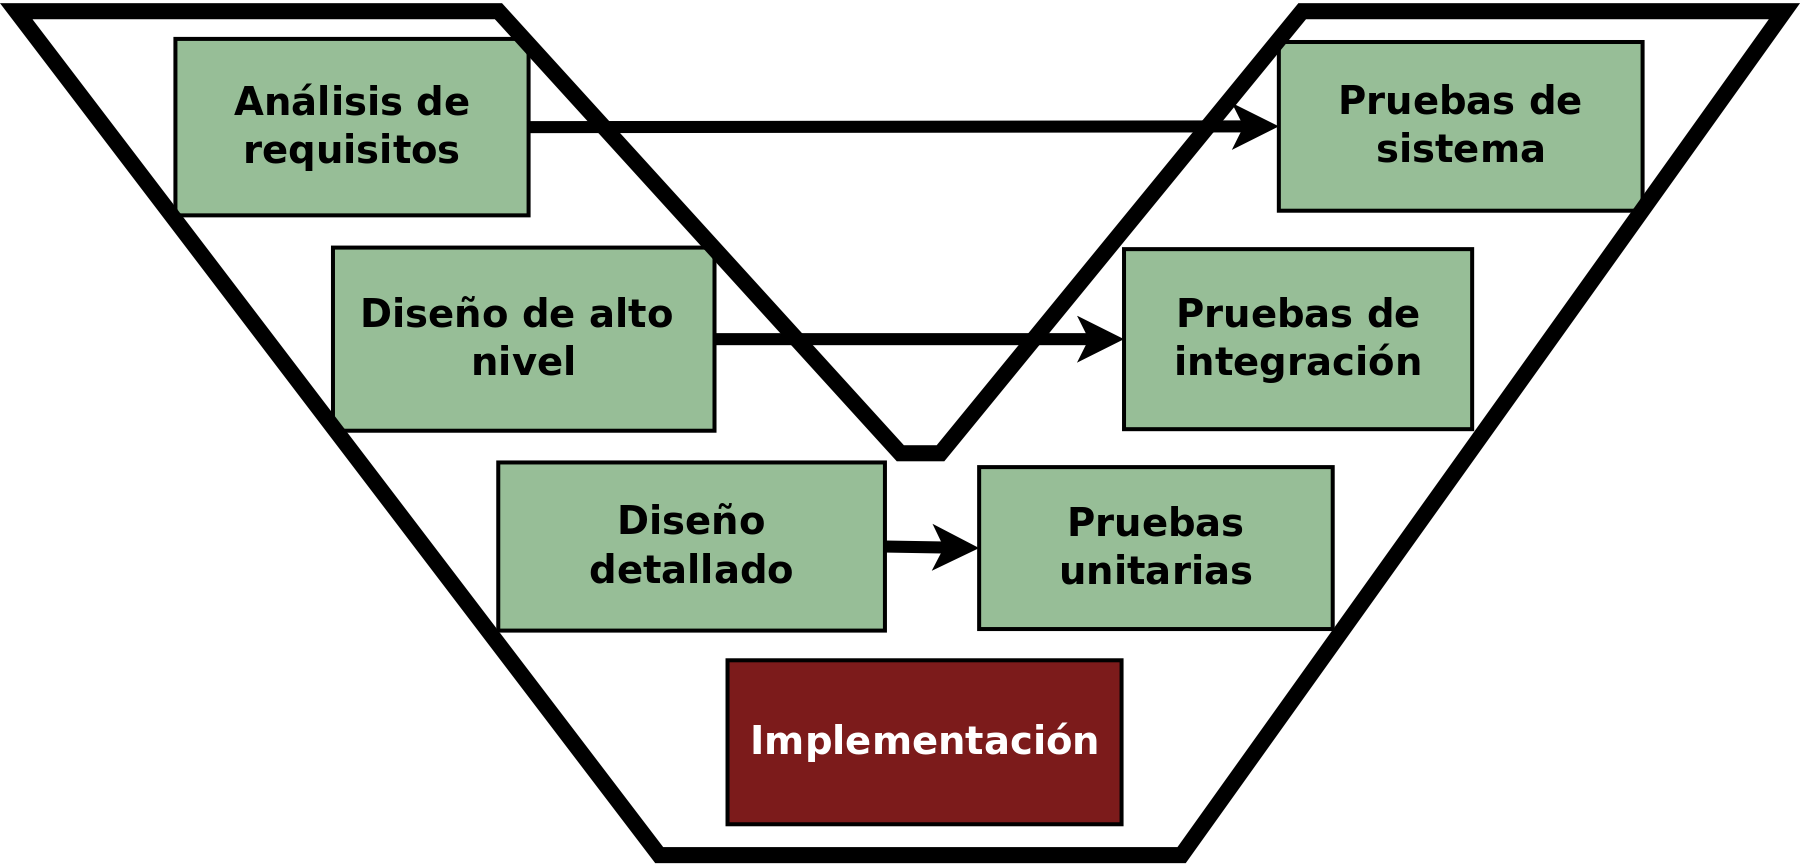
\includegraphics[width=\textwidth]{./Figures/modeloV.png}
	\caption{Modelo de desarrollo y validación en V}
	\label{fig:modeloV}
\end{figure}

A continuación se pone en relieve cada una de estas instancias del proceso de desarrollo.

\subsection{Analisis de los requerimientos}

A partir de un análisis de los requerimientos explicitados en el capítulo anterior se puede determinar que los Requerimientos 1 y 2 están estrictamente asociados al hardware. Se puede ligar alguno de estos requerimientos al firmware, como por ejemplo el R1.1 ya que el firmware es el responsable de la entrada a modos de bajo consumo o la administración de energía dentro del microcontrolador. Sin embargo, la mayor carga de responsabilidad de cumplimiento de estos requerimientos están volcados sobre el hardware. Los requerimientos 3 y 4 están muy ligados al desarrollo del firmware del equipo. Solamente el requerimiento 4.2 está relacionado al tamaño de la memoria utilizada que es una cuestión de hardware.

Una vez iniciado el proceso de desarrollo se notó que la lista de requerimientos del capítulo anterior no es exhaustiva y da por supuesto las funcionalidades básicas del equipo. Se procedió entonces a elaborar una serie de requerimientos más específicos sobre el funcionamiento detallado de la operación del usuario y los parámetros que es posible configurar, que permita luego asociar requisitos puntuales a los casos de uso del equipo. 

\textbf{Requerimientos adicionales :}

\begin{enumerate}

	\setcounter{enumi}{4}

	\item \textbf{Requerimientos estructurales:} 
	\begin{enumerate}[label*=\arabic*.]
		\item El equipo debe poder adquirir señales analógicas de hasta dos canales de entrada.
		\item El desfasaje entre las señales adquiridas debe ser nulo.
		\item El equipo debe inicializar solamente los periféricos que se utilicen en el momento adecuado para ahorrar energía. 
	\end{enumerate}
	
	\item \textbf{Requerimientos operativos:}
	\begin{enumerate}[label*=\arabic*.]
		\item Al estar inactivo, el equipo debe entrar en modo configuración para poder ponerse en hora y mantenerla mientras tenga batería.
		\item Al estar en configuración, se debe poder chequear el correcto funcionamiento del hardware (SD, conversor AD, etc).
		\item Si el equipo esta inactivo, al enviar un comando desde la terminal, se comienza a adquirir y enviar vía bluetooth (esta señal puede estar decimada y con menor resolución) con la configuración previamente seleccionada.
		\item Si el equipo está adquiriendo y enviando vía bluetooth, se puede enviar una orden para que el equipo finalice y vuelva al modo inactivo.
		\item Si el equipo está adquiriendo y enviando vía bluetooth, se puede enviar una orden para que el equipo comience a almacenar en la memoria SD.
		\item Si se esta adquiriendo, enviando señal vía bluetooth y almacenando en la SD, se debe poder enviar una orden para que el equipo deje de hacerlo y vuelva al modo inactivo.
		\item Si se esta adquiriendo, almacenando y enviando por Bluetooth, se debe poder enviar una orden para que el equipo deje de enviar la señal por Bluetooth y continúe la experiencia en forma silenciosa.
		\item Si el equipo está adquiriendo y almacenando en forma silenciosa, se debe poder enviar un comando para que vuelva a enviar la señal por Bluetooth sin interrumpir ni alterar la adquisición y almacenamiento.
		\item Si el equipo está adquiriendo, enviando señal via Bluetooth y almacenando, se puede enviar un comando para que el equipo deje almacenar.
		\item Si el equipo esta inactivo, se puede requerir el envío de una señal patrón para chequeo del canal de comunicación.
		\item Si el equipo esta enviando la señal patrón para chequeo de canal de comunicación, se puede enviar un comando para que el equipo vuelva a modo inactivo.
		\item Se debe almacenar por cada registro la hora, los canales activados y el nivel de batería.
		\item Cada vez que se comienza un nuevo almacenamiento, se genera un archivo nuevo con nombre auto numerado.
		\item Cada vez que comienza o finaliza un almacenamiento, se registra en un archivo que debe contener el nombre del archivo y la fecha y hora de inicio y fin de todas las experiencias.
		\item Cada uno de estos modos debe estar señalizado por uno o mas leds para comprobar visualmente el funcionamiento.
	\end{enumerate}
	
	\item \textbf{Requerimientos de configuración}
	
	\begin{enumerate} [label*=\arabic*.]
		\item El equipo debe tener una configuración por default y la posibilidad de modificarla mientras no se esta adquiriendo.
		\item El equipo debe poder volver a la configuración de fábrica.
		\item El equipo debe guardar la última configuración y utilizarla.
		\item Se debe poder elegir la frecuencia de muestreo dentro de algunas opciones.
		\item Se debe poder elegir si activar uno o los dos canales.
		\item Se debe poder elegir la ganancia del amplificador.
		\item El equipo se debe poder calibrar con dos puntos de presión conocidos.		
	\end{enumerate}


\end{enumerate}

\textbf{Casos de Uso:}

De toda la lista completa de requerimientos surgen los casos de uso con operaciones básicas del usuario. A continuación se muestran los diferentes casos de uso que se desprenden de los requerimientos:

	\underline{Caso de uso CU0001:}

	\begin{enumerate} 
		\item Nombre: CU0001
		\begin{enumerate} [label*=\arabic*.]
			\item Descripción: Autonomía
			\item Actor Principal: Usuario
			\item Disparador: Encendido del equipo		
		\end{enumerate}
		\item Flujo de eventos
		\begin{enumerate} [label*=\arabic*.]
			\item Flujo básico: el usuario enciende el equipo, realiza la configuración y comienza la experiencia. Luego de 24 hs finaliza la experiencia desde una terminal.
			\item Flujo alternativo: Si la batería no tiene carga total, es responsabilidad del usuario. Según la configuración se puede calcular autonomía aproximada.
		\end{enumerate}

		\item Requerimientos especiales: conexión Bluetooth
		\item Pre-condiciones: cargar la batería al 100\% antes de comenzar a usar el equipo.
		\item Post-Condiciones: Finalizar correctamente la experiencia.				
	\end{enumerate}

	\underline{Caso de uso CU0002:}

	\begin{enumerate} 
		\item Nombre: CU0002
		\begin{enumerate} [label*=\arabic*.]
			\item Descripción: Configuración
			\item Actor Principal: Usuario
			\item Disparador: Ingreso a configuración desde la terminal
		\end{enumerate}
		\item Flujo de eventos
		\begin{enumerate} [label*=\arabic*.]
			\item Flujo básico: el usuario desde la terminal ingresa al modo configuración, modifica los parámetros que necesita o calibra un canal, y vuelve a salir del modo configuración.
			\item Flujo alternativo:
			\begin{itemize}
				\item Si el equipo no está sincronizado, indica error y da la oportunidad de reiniciar. 
				\item Si no se puede abrir la última configuración, debe abrir la configuración de fábrica y mostrar error.
				\item La nueva configuración elegida se guarda y se comprueba al comenzar la experiencia. Hasta ese momento no se comprueba si es correcta.
				\item Si se comprueba algún error de hardware, se debe enviar un mensaje de reparación.						
			\end{itemize}				
		\end{enumerate}

		\item Requerimientos especiales: conexión Bluetooth
		\item Pre-condiciones: equipo en modo inactivo
		\item Post-Condiciones: salir correctamente del modo configuración.
	\end{enumerate}



	\underline{Caso de uso CU0003:}

	\begin{enumerate} 
		\item Nombre: CU0003
		\begin{enumerate} [label*=\arabic*.]
			\item Descripción: Experiencia
			\item Actor Principal: Usuario
			\item Disparador: Ingreso a experiencia desde la terminal
		\end{enumerate}
		\item Flujo de eventos
		\begin{enumerate} [label*=\arabic*.]
			\item Flujo básico: el usuario desde la terminal ingresa al modo de adquisición y visualización, comprueba el correcto funcionamiento de los sensores habilitados observando la señal adquirida. Luego ingresa al modo almacenamiento y comprueba que no haya error en el almacenamiento de datos. Luego selecciona dejar de enviar para que la experiencia continúe en modo silencioso. Al finalizar la experiencia, el usuario envía la orden para terminar la adquisición. El usuario luego comprueba que la adquisición fue completa.
			\item Flujo alternativo:
			\begin{itemize}
				\item Si los sensores no muestran una señal adecuada, se debe salir de la adquisición y chequear conectores.
				\item Si los sensores no muestran ninguna señal, se debe comprobar el canal.
				\item Si hay error al comenzar a almacenar, se detiene la adquisición para comprobar el funcionamiento de la tarjeta SD.
				\item Si se necesita ver las señales por una eventual desconexión, se puede conectar mediante bluetooth para visualizar las señales y luego salir. 
				\item Si no se puede volver a conectar con la terminal, se debe acceder físicamente a conectar el equipo a una PC.
				\item Si la batería esta en un nivel crítico, el equipo debe guardar el archivo y finalizar la experiencia. El usuario se notifica de esto al intentar conectarse.					
			\end{itemize}				
		\end{enumerate}

		\item Requerimientos especiales: conexión Bluetooth
		\item Pre-condiciones: equipo en modo inactivo
		\item Post-Condiciones: salir correctamente de la experiencia.
	\end{enumerate}


	\underline{Caso de uso CU0004:}

	\begin{enumerate} 
		\item Nombre: CU0004
		\begin{enumerate} [label*=\arabic*.]
			\item Descripción: Experiencia
			\item Actor Principal: Usuario
			\item Disparador: Ingreso a experiencia desde la terminal
		\end{enumerate}
		\item Flujo de eventos
		\begin{enumerate} [label*=\arabic*.]
			\item Flujo básico: el usuario desde la terminal ingresa al modo de adquisición y visualización, comprueba el correcto funcionamiento de los sensores habilitados observando la señal adquirida. Luego ingresa al modo almacenamiento y comprueba que no haya error en el almacenamiento de datos. Luego selecciona dejar de enviar para que la experiencia continúe en modo silencioso. Al finalizar la experiencia, el usuario envía la orden para terminar la adquisición. El usuario luego comprueba que la adquisición fue completa.
			\item Flujo alternativo:
			\begin{itemize}
				\item Si los sensores no muestran una señal adecuada, se debe salir de la adquisición y chequear conectores.
				\item Si los sensores no muestran ninguna señal, se debe comprobar el canal.
				\item Si hay error al comenzar a almacenar, se detiene la adquisición para comprobar el funcionamiento de la tarjeta SD.
				\item Si se necesita ver las señales por una eventual desconexión, se puede conectar mediante bluetooth para visualizar las señales y luego salir. 
				\item Si no se puede volver a conectar con la terminal, se debe acceder físicamente a conectar el equipo a una PC.
				\item Si la batería esta en un nivel crítico, el equipo debe guardar el archivo y finalizar la experiencia. El usuario se notifica de esto al intentar conectarse.					
			\end{itemize}				
		\end{enumerate}

		\item Requerimientos especiales: conexión Bluetooth
		\item Pre-condiciones: equipo en modo inactivo
		\item Post-Condiciones: salir correctamente de la experiencia.
	\end{enumerate}

	\underline{Caso de uso CU0005:}

	\begin{enumerate} 
		\item Nombre: CU0005
		\begin{enumerate} [label*=\arabic*.]
			\item Descripción: Descarga de datos y carga de batería.
			\item Actor Principal: Usuario
			\item Disparador: Conectar el equipo por USB a PC
		\end{enumerate}
		\item Flujo de eventos
		\begin{enumerate} [label*=\arabic*.]
			\item Flujo básico: el usuario conecta el equipo a la PC y comprueba que se reconozca como un medio de almacenamiento masivo. Luego descarga los archivos que sean necesarios y deja el equipo conectado mientras necesite cargar la batería. Finalmente, luego de finalizadas todas las transferencias de datos, desconecta el equipo del USB.
			\item Flujo alternativo:
			\begin{itemize}
				\item Si la PC no reconoce al equipo como medio de almacenamiento masivo, se debe comprobar la tarjeta SD.
				\item Si el equipo no carga la batería, se debe hacer una revisión técnica del equipo y de las baterías.			
			\end{itemize}				
		\end{enumerate}

		\item Requerimientos especiales: conexión USB
		\item Pre-condiciones: equipo en modo inactivo
		\item Post-Condiciones: desconectar el USB cuando no haya ninguna transferencia activa y cuando haya terminado de cargar la batería. El nivel de batería se puede comprobar desde la terminal entrando al modo configuración.
	\end{enumerate}
	
A partir de los requerimientos y casos de usos armamos la matriz de trazabilidad, que consiste en una tabla de doble entrada que asocia cada requerimiento con uno o más casos de uso.

\footnotesize
\begin{longtable}[c]{lllllll}
\hline
\textbf{REQ/CU} & \textbf{CU0001} & \textbf{CU0002} & \textbf{CU0003} & \textbf{CU0004} & \textbf{CU0005} & \textbf{Ensayo} \\ \hline
\endhead
%
R1.1 & X &  &  &  &  & \begin{tabular}[c]{@{}l@{}}Comprobación post-experiencia\\ 			Medición de corriente consumida\end{tabular} \\ \hline
R1.2 &  &  &  &  &  & Conexión desde terminal \\ \hline
R2.1 &  &  &  &  &  & Pesaje del equipo \\ \hline
R2.2 &  &  &  &  &  & Medición del equipo \\ \hline
R2.3 &  &  &  &  &  & Medición temperatura \textless 40º \\ \hline
R3.1 &  &  & X &  &  & Test MDE \\ \hline
R3.2 &  &  & X &  &  & Test MDE \\ \hline
R3.3 &  & X &  &  &  & Comprobación post-experiencia \\ \hline
R3.4 &  &  &  &  & X & Test conexión PC \\ \hline
R4.1 &  &  & X &  &  & Test Calibración \\ \hline
R4.2 &  &  & X &  & X & \begin{tabular}[c]{@{}l@{}}Test conexión PC\\ 			Comprobación post-experiencia\end{tabular} \\ \hline
R4.3 &  &  &  &  & X & Comprobación post-experiencia \\ \hline
R5.1 &  &  & X &  &  & Comprobación post-experiencia \\ \hline
R5.2 &  &  & X &  &  & Comprobación post-experiencia \\ \hline
R5.3 &  &  &  &  &  & Medición de corriente consumida \\ \hline
R6.1 &  &  & X &  &  & Test MDE \\ \hline
R6.2 &  &  & X &  &  & Test MDE \\ \hline
R6.3 &  &  & X &  &  & Test MDE \\ \hline
R6.4 &  &  & X &  &  & Test MDE \\ \hline
R6.5 &  &  & X &  &  & Test MDE \\ \hline
R6.6 &  &  & X &  &  & Test MDE \\ \hline
R6.7 &  &  & X &  &  & Test MDE \\ \hline
R6.8 &  &  & X &  &  & Test MDE \\ \hline
R6.9 &  &  & X &  &  & Test MDE \\ \hline
R6.10 &  &  &  & X &  & Test MDE \\ \hline
R6.11 &  &  &  & X &  & Test MDE \\ \hline
R6.12 &  &  & X &  & X & Comprobación post-experiencia \\ \hline
R6.13 &  &  & X &  & X & Comprobación post-experiencia \\ \hline
R6.14 &  &  &  &  & X & Comprobación post-experiencia \\ \hline
R6.15 &  &  & X &  &  & Comprobación visual \\ \hline
R7.1 &  & X &  &  &  & Comprobación post-experiencia \\ \hline
R7.2 &  & X &  &  &  & Comprobación post-experiencia \\ \hline
R7.3 &  & X &  &  &  & Comprobación post-experiencia \\ \hline
R7.4 &  & X &  &  &  & Comprobación post-experiencia \\ \hline
R7.5 &  & X &  &  &  & Comprobación post-experiencia \\ \hline
R7.6 &  & X &  &  &  & Comprobación post-experiencia \\ \hline
\caption{Matriz de Trazabilidad}
\label{tab:matrizTrazabilidad}\\
\end{longtable}

\normalsize


\subsection{Diseño de alto nivel}

Una vez especificados y analizados todos los requerimientos, se da a lugar al diseño del sistema en alto nivel, es decir, analizar los subsitemas que lo conforman y su relación entre sí. Los subsistemas que entran en juego son los siguientes:

\footnotesize
\begin{tabularx}{\textwidth}{XXXX}
\hline
\textbf{Subsistema} & \textbf{Responsabilidad} & \textbf{Entrada} & \textbf{Salida} \\ \hline
Sensores & Sensar señal de presión & Señal física de presión & Señal analógica \\ \hline
Acondicionamiento analógico & Filtrar y ajustar ganancia de señal analógica & Señal analógica de presión & Señal analógica de presión acondicionada \\ \hline
ADS1292 & Adquirir señal analógica & Señal analógica de presión acondicionada & Señal digital via SPIPin Data Ready \\ \hline
SD & Almacenar señal adquirida & Paquete de muestras de señales adquiridas & Archivos csv con muestras y archivo con registro de actividad \\ \hline
Led & Indicadores de estado & Niveles lógicos & Encendido o apagado como indicador \\ \hline
Sistema de alimentación y carga de batería & - Cargar la batería al conectar por USB- Alimentar el sistema al no tener conectado el USB a partir de la batería & Tensión USB o de batería & -Corriente de alimentación de USB - Tensión regulada \\ \hline
USB & - proveer tensión para carga de batería- conectividad a PC via medio de almacenamiento masivo & Conector USB a PC & Visualización de sistemas de archivos interna \\ \hline
Bluetooth & Conectividad con terminal & Comandos vía BT & Comandos y datos vía BT \\ \hline
\caption{Subsistemas del equipo}
\label{tab:subsistemas}\\
\end{tabularx}
\normalsize

Los subsistemas de la tabla anterior son los bloques básicos desde de los cuales se conforma el dispositivo. Es necesario recurrir a patrones de diseño para articular entre sí los diferentes módulos.

\textbf{Patrones de Diseño:}

En primer lugar, la cadena de adquisición, envío de datos y almacenamiento se asocia a un patrón productor/consumidor, donde el conversor analógico digital ADS1292 y ADC interno son los productores de datos, y las salidas por Bluetooth y almacenamiento en la SD son los consumidores. a información producida se guarda en un ping-pong buffer \citep{zhou2017} del cual leen las demás tareas. Esto puede visualizarse en la figura \ref{fig:patronProdCons}.

En este patrón también participa el esquema de "\textit{proxy pattern}" \citep{douglass2011}, que se refiere a un esquema de funcionamiento en el que un elemento de software es el responsable del acceso a un recurso de hardware, y todas las tareas que quieran acceder al recurso lo hacen a través de este elemento. Se utiliza una estructura o clase que encapsule todos los accesos al hardware, sin importar su interfaz física. Este proxy publica los servicios que permiten leer y escribir en el dispositivo, así como inicializar, configurar y apagar el dispositivo. En el diagrama de la figura \ref{fig:patronProdCons} pueden verse en verde todos los elementos de hardware, y con flechas la interfaz física través del cual se comunica. 

\begin{figure}[!htbp]
	\centering
	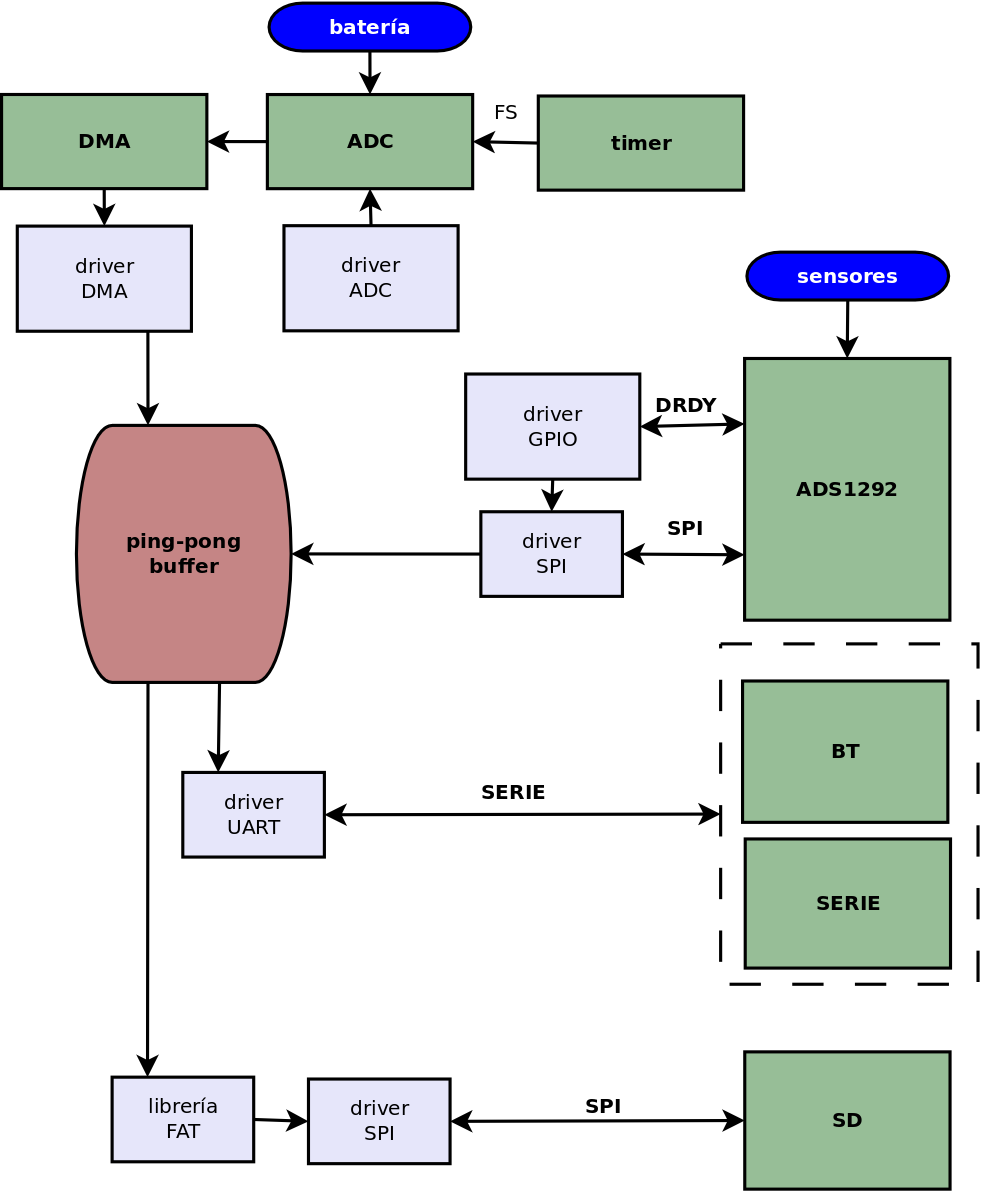
\includegraphics[width=\textwidth]{./Figures/patronProdCons.png}
	\caption{Diagrama de relaciones entre subsistemas. Patrón productor/consumidor}
	\label{fig:patronProdCons}
\end{figure}

Los módulos de hardware que se muestran en la figura \ref{fig:patronProdCons} son los siguientes:

\begin{itemize}
	\item ADS1292: se trata de un conversor analógico digital de alta resolución (24 bits), con dos canales de entrada diferencial simultáneos, de tecnología Sigma-Delta. Incluye internamente un amplificador de ganancia programable (PGA). Puede trabajar a una frecuencia de muestreo máxima de 8kSPS. La interfaz de comunicación es a través de un bus SPI \citep{texas2012} . El conversor tiene dos modos de operación: puede indicar con el pin DRDY que cuenta con datos a ser leídos y esperar el comando RDATA, o puede estar en el modo “Read Data Continous” (RDATAC) y enviar comandos constantemente. En el diagrama anterior se muestra la conexión a través del pin DRDY para mostrar el caso general y ser compatible con cualquiera de los dos modos de envío de datos.
	\item Bluetooth: la conexión bluetooth se realiza a través de un módulo HC-06. Se conecta al microcontrolador a través de un puerto serie y permite la comunicación entre el software de la terminal y la aplicación guardada en el firmware. Cuenta con un pin de habilitación y una salida de STATE para indicar cuando hay vigente una conexión bluetooth.
	\item Serie: solamente se utiliza para desarrollo y pruebas de comunicación. Físicamente se trata de un conversor USB-TTL y se maneja a través de un driver de la UART.
	\item SD: el medio de almacenamiento masivo del dispositivo es una tarjeta microSD. La placa cuenta con un slot de microSD que permite la conexión entre la tarjeta y el microcontrolador a través de un bus SPI, además de un pin que permite detectar cuando hay una tarjeta conectada. La interfaz entre la aplicación y el hardware se hace en dos capas: la aplicación se comunica con el nivel de manejo de archivos (librería FatFs), y esta librería se comunica con las funciones del driver SPI \citep{chan2014}, como se visualiza en la figura \ref{fig:capasFatFs}.
	
\begin{figure}[!htbp]
	\centering
	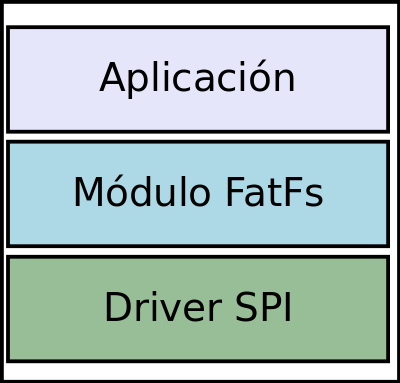
\includegraphics[width=\textwidth]{./Figures/capasFatFs.png}
	\caption{Capas de software de la librería FatFs}
	\label{fig:capasFatFs}
\end{figure}	
	
	\item ADC: se trata de un conversor analógico digital interno al microcontrolador, de 12 bits de resolución, 8 canales multiplexados, de tecnología SAR (aproximaciones sucesivas). Se habilita la conversión a través de la habilitación de un timer que temporiza la frecuencia de muestreo. Los resultados de la conversión del ADC se transfieren a memoria a través del DMA.
	\item DMA: uno de los canales está configurado en modo “PERIPHERAL TO MEMORY”, realizando las transferencias entre el periférico ADC y un puntero que apunta a un buffer. En cada transferencia el puntero se incrementa hasta llegar al final y generar una interrupción. 
\end{itemize}

\subsection{Diseño Detallado}

En base al diseño de alto nivel realizado anteriormente, se da a lugar al diseño detallado de los elementos del programa como tareas y máquinas de estado.

\textbf{Diseño de tareas}

El firmware está basado en un sistema operativo de tiempo real, específicamente en el freeRTOS \citep{aws2017}.  En el diagrama de la figura \ref{fig:tareasCompleto} se puede observar un esquema detallado de las tareas involucradas y sus relaciones entre ellas. Cada una de las filas del gráfico corresponde a un nivel de prioridad, siendo “cero” el nivel de menor prioridad y “cuatro” el de máxima prioridad utilizado. El nivel “IRQ” corresponde a las rutinas de atención de interrupción, que en el sistema freeRTOS tienen una prioridad siempre mayor a cualquiera de las tareas. En verde se pueden ver los mecanismos de comunicación entre tareas, como semáforos o colas de datos. Las flechas que no tienen ninguna indicación corresponden a flags, estados o asignación directa de variables de menor complejidad. 

\begin{adjustbox}{center,caption={Diagrama de tareas completo},label={fig:tareasCompleto},nofloat=figure,vspace=\bigskipamount}
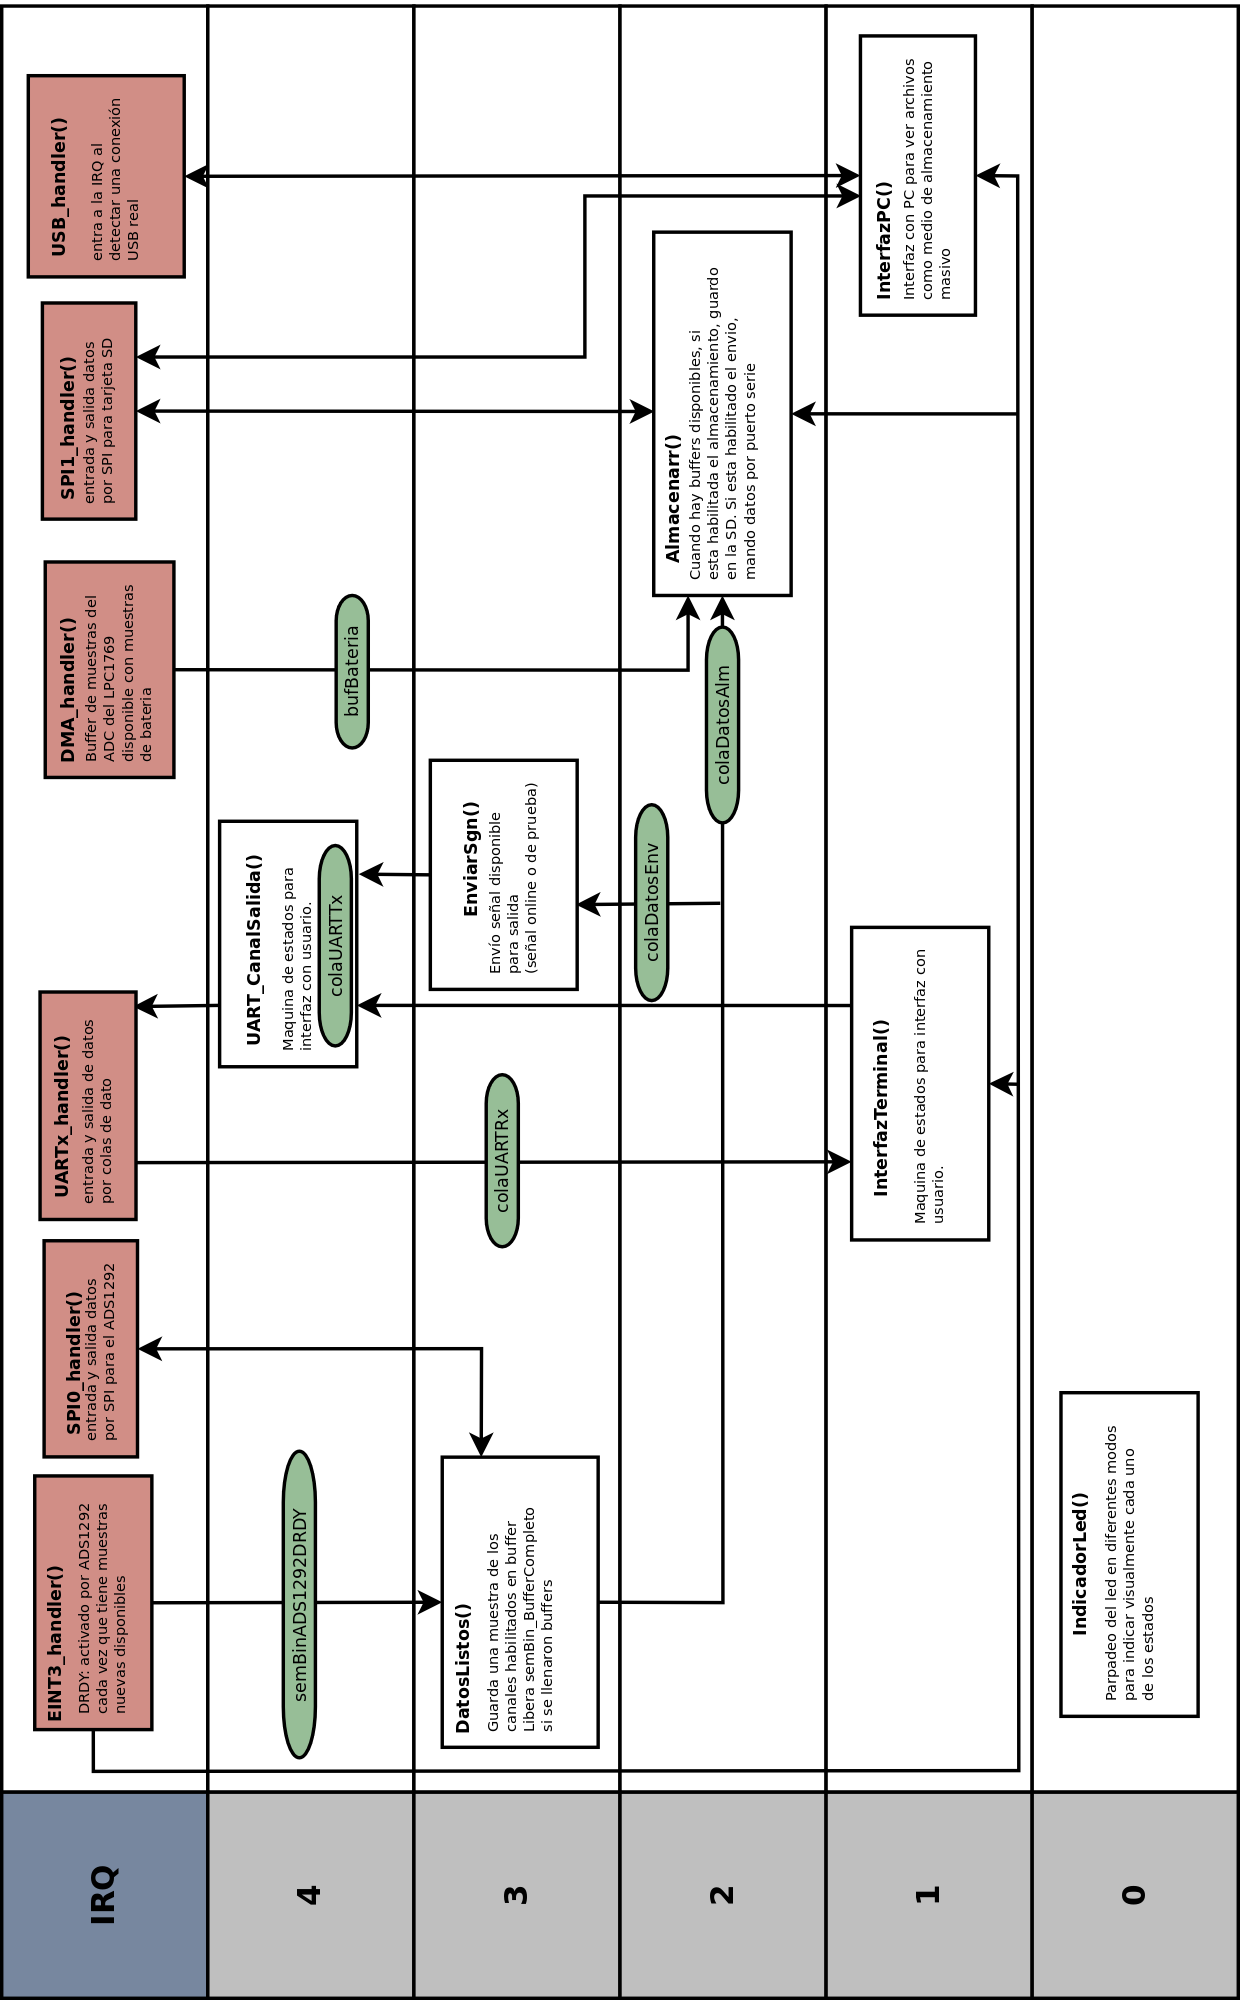
\includegraphics[scale = 0.24]{./Figures/tareasCompleto.png}
\end{adjustbox}
	
Este diagrama explica en gran detalle el funcionamiento del firmware. En el nivel de prioridad 1 se encuentran las tareas de interfaz con el usuario, que son de menor prioridad porque no tienen una exigencia crítica de tiempo. Se explica a continuación el funcionamiento en diferentes casos:

\begin{itemize}

	\item Al iniciar el equipo, solo está activa la tarea “InterfazTerminal()”, que es la encargada de comunicarse con el usuario remoto respetando el diagrama de estados de la figura \ref{fig:tareasInactivo}. En este caso solamente intervienen esta tarea, la tarea UART\_CanalSalida(), que es una tarea cercana al hardware que hace la interfaz entre la cola de datos de salida y el registro de la UART, y finalmente la propia rutina de interrupción de la UART que escribe en la cola de datos de entrada cada vez que recibe un mensaje, y envía los datos de salida permitiendo escribirse en bloques hasta del tamaño de la FIFO interna del periférico (16 bytes). En nivel de prioridad cero siempre se ejecuta una tarea que señaliza con parpadeo de leds según el modo de funcionamiento activo. En este caso, es un parpadeo cada 500ms.

\begin{adjustbox}{center,caption={Diagrama de tareas en modo inactivo},label={fig:tareasInactivo},nofloat=figure,vspace=\bigskipamount}
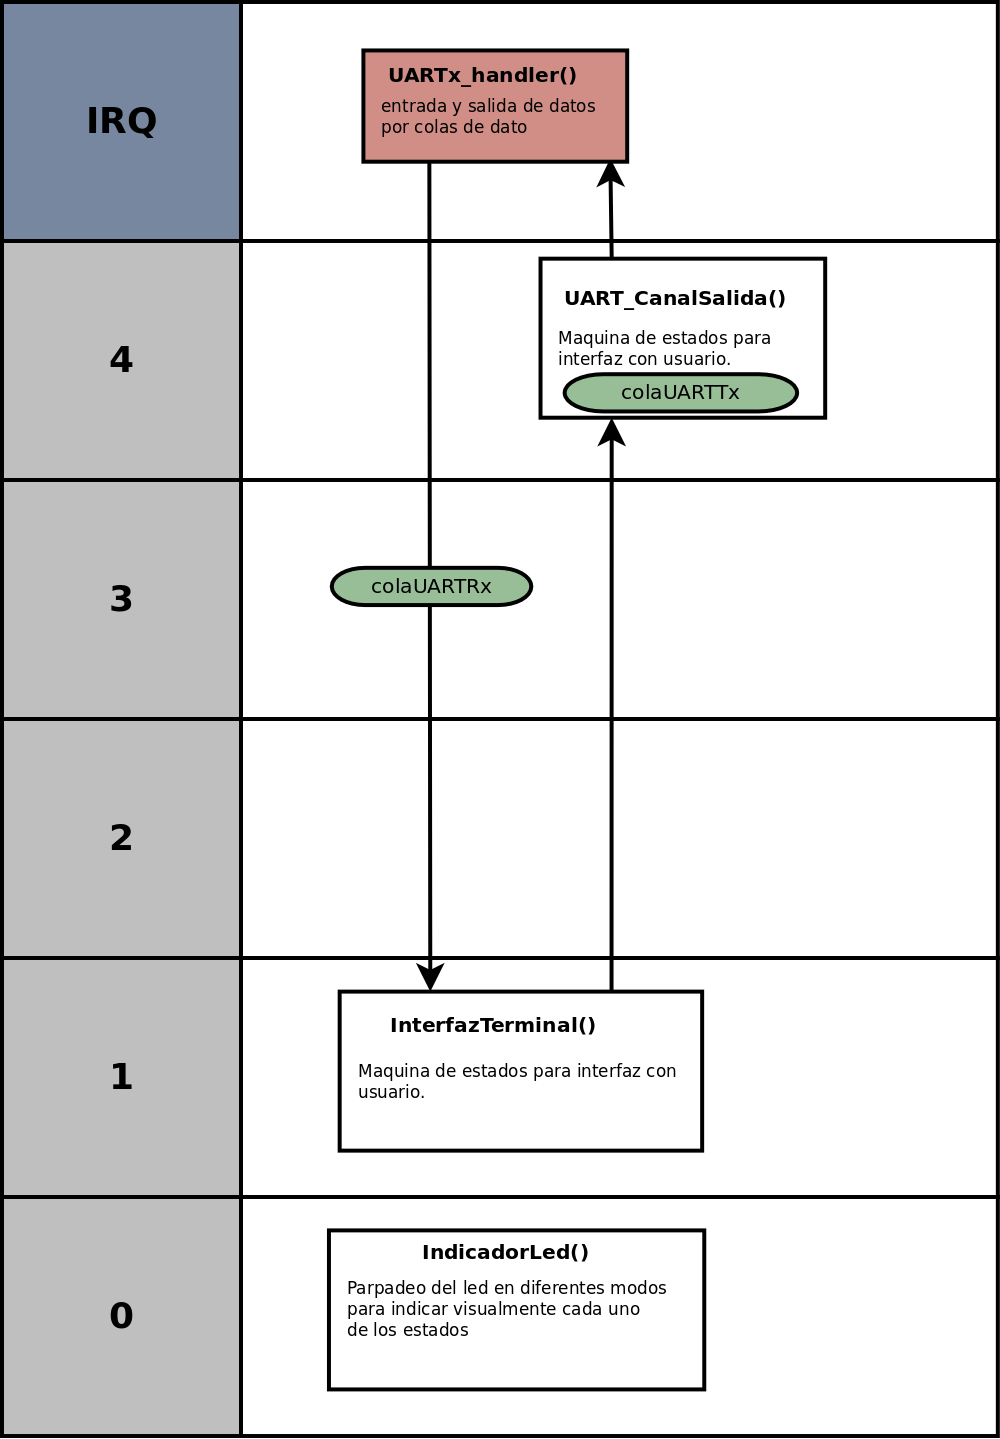
\includegraphics[scale = 0.17]{./Figures/tareasInactivo.png}
\end{adjustbox}

	\item Cuando el equipo pasa al modo “adquirir+enviar”, se inicializa el hardware de adquisición (ADS1292), que se comunica a través del bus SPI0 y de una entrada de propósito general (GPIO) conectada al pin DRDY. Como se explicó anteriormente, uno de los modos de funcionamiento del ADS1292 es señalizar a través del pin DRDY la disponibilidad de datos nuevos para ser leídos. La rutina de interrupción de GPIO “EINT3\_handler()” se activa en cada nivel bajo del pin DRDY, y libera el semáforo “semBinADS1292DRDY”. Por otro lado, esto libera la tarea “DatosListos()” que se encontraba en estado bloqueado en espera de este semáforo, para luego enviar el comando RDATA a través del bus SPI, y recibir finalmente el dato leído para almacenarlo en un buffer. 

		Al ingresar a este modo, se instala una tarea llamada “EnviarSgn()”, que se encuentra bloqueada a través de la cola de datos “colaDatosEnv”. La tarea “DatosListos()” envía un puntero a buffer a través de esta cola de datos cada vez que se completa un buffer de adquisición, de manera que la tarea “EnviarSgn()” también escriba en la cola de datos de salida de la UART, “colaUART”.
		
\begin{adjustbox}{center,caption={Diagrama de tareas en modo adquirir y enviar},label={fig:VOP24_tareas_v1_adquirirEnviar},nofloat=figure,vspace=\bigskipamount}
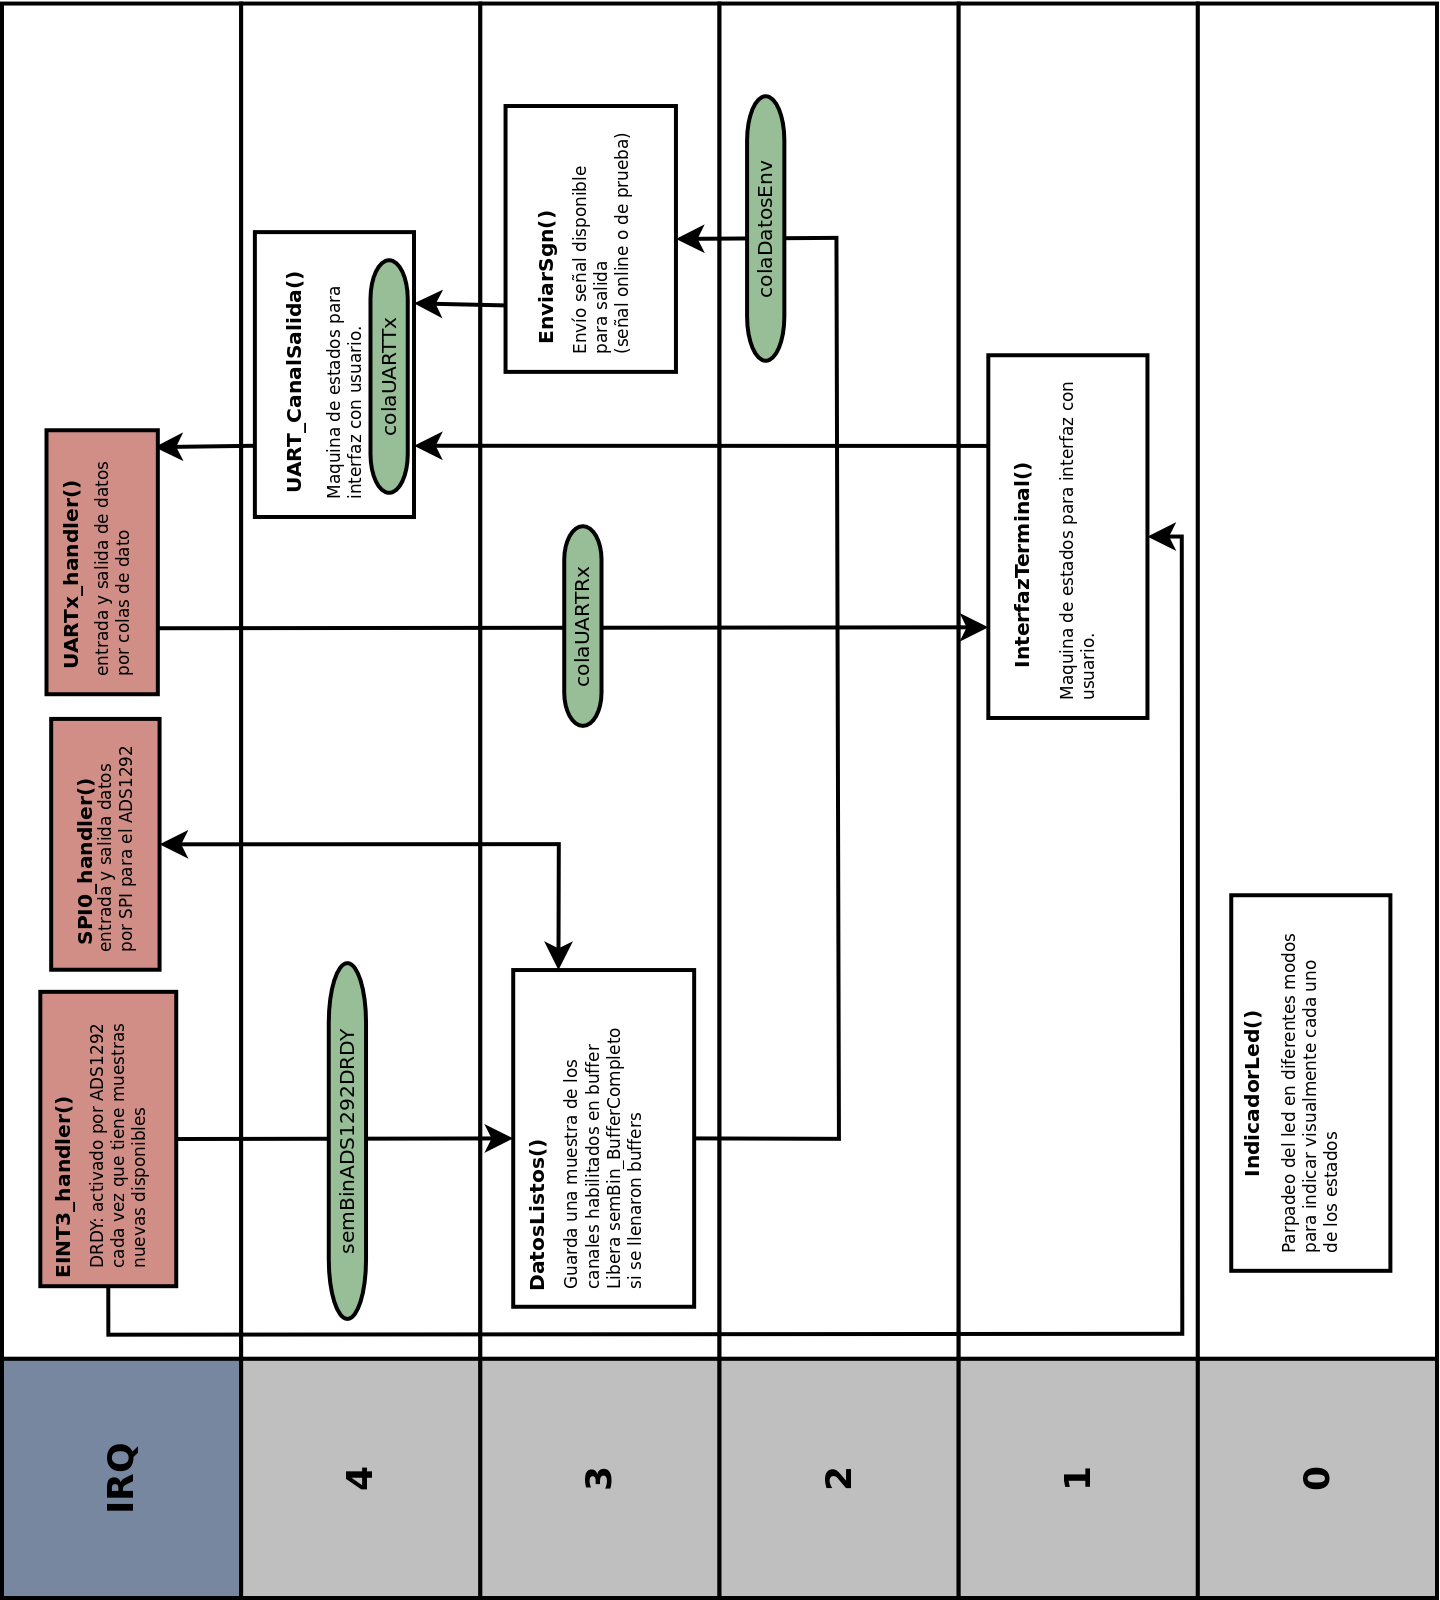
\includegraphics[scale = 0.23]{./Figures/VOP24_tareas_v1_adquirirEnviar.png}
\end{adjustbox}		
		
	\item Al ingresar al modo “adquirir+enviar+almacenar”, se agrega la tarea “Almacenar()”, que también se encuentra bloqueada a través de una cola de datos llamada “colaDatosAlm”, a través de la cual se envía un puntero a buffer a ser guardado en la memoria SD. 
	
\begin{adjustbox}{center,caption={Diagrama de tareas en modo adquirir, enviar y almacenar},label={fig:VOP24_tareas_v1_adquirirEnviarAlmacenar},nofloat=figure,vspace=\bigskipamount}
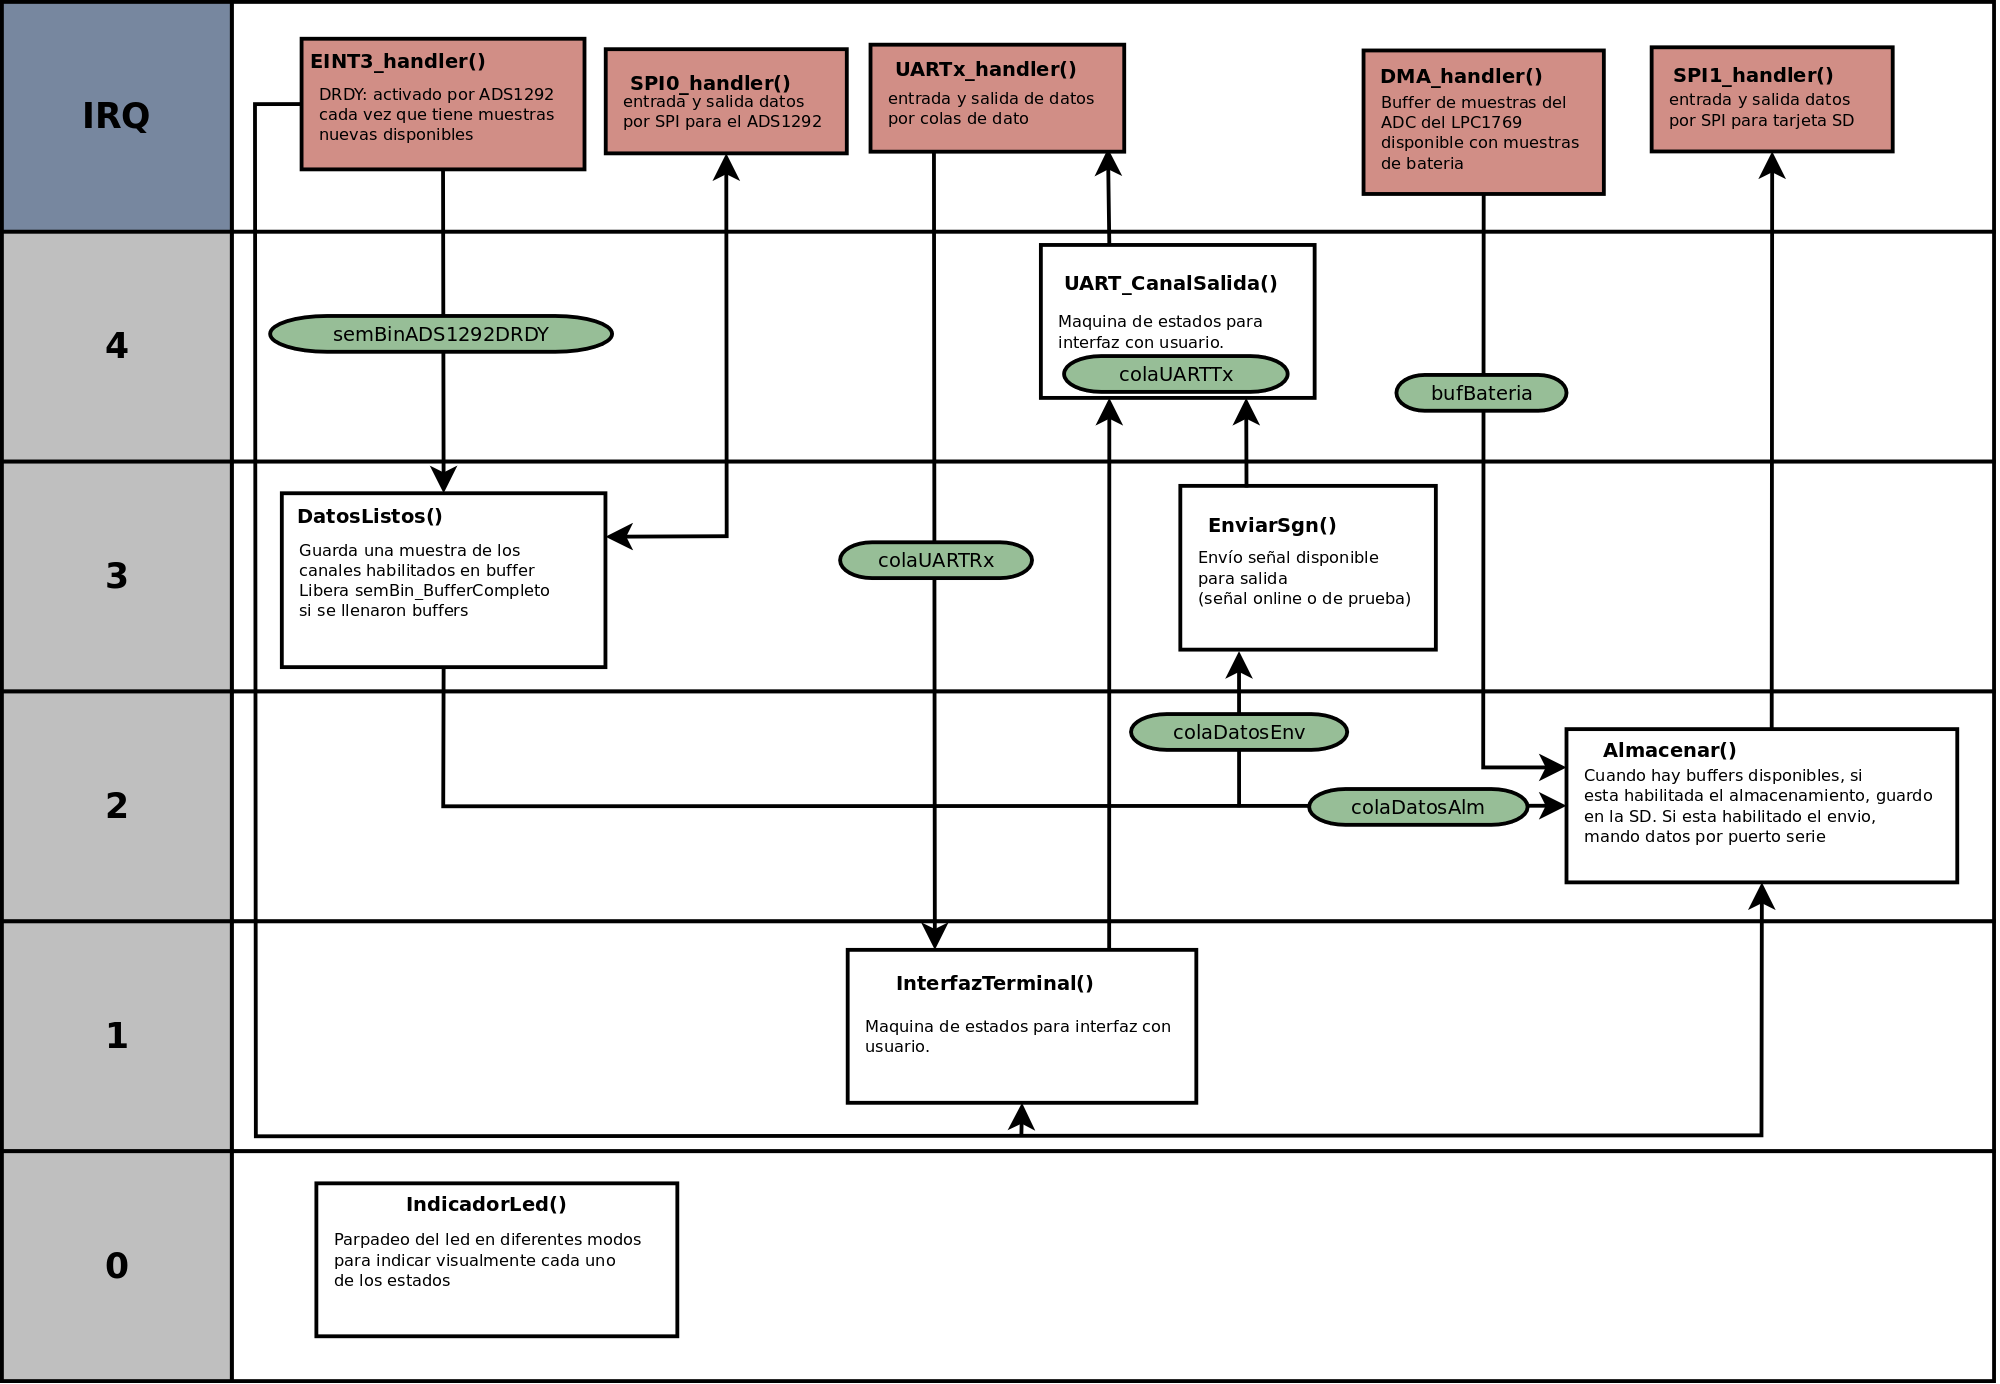
\includegraphics[angle= 90, scale = 0.20]{./Figures/VOP24_tareas_v1_adquirirEnviarAlmacenar.png}
\end{adjustbox}
	
	La tarea Almacenar() se comunica a través de un bus SPI directamente con la tarjeta SD. El tamaño del buffer de almacenamiento se definió haciendo pruebas entre el tiempo de llenado del buffer (cantidad de muestras multiplicado por período de muestreo) versus el tiempo de almacenamiento que demora escribir el buffer como archivo en la memoria SD. Este último tiempo no es lineal a la cantidad de muestras, por lo que se hicieron varias pruebas hasta determinar un tamaño óptimo para el peor caso que es la máxima frecuencia de muestreo posible. El tamaño determinado es de 1024 muestras y se comprobó a 500 muestras por segundo con dos canales habilitados. 
	
Al almacenar en la SD también se guardan las muestras de medición de batería. Para ello se hace un promedio de una ráfaga de muestras que se guardan en un buffer “bufBateria” a través del DMA.

	\item Durante el modo “adquirir+almacenar” se suspende la tarea “EnviarSgn()” y el resto de las tareas continúa igual. El led pasa a realizar dos parpadeos en un segundo y luego permanece apagado el siguiente segundo. Esta es la indicación visual de que el equipo se encuentra correctamente funcionando mientras el usuario no tenga acceso mediante bluetooth.


\begin{adjustbox}{center,caption={Diagrama de tareas en modo adquirir y almacenar},label={fig:VOP24_tareas_v1_adquirirAlmacenar},nofloat=figure,vspace=\bigskipamount}
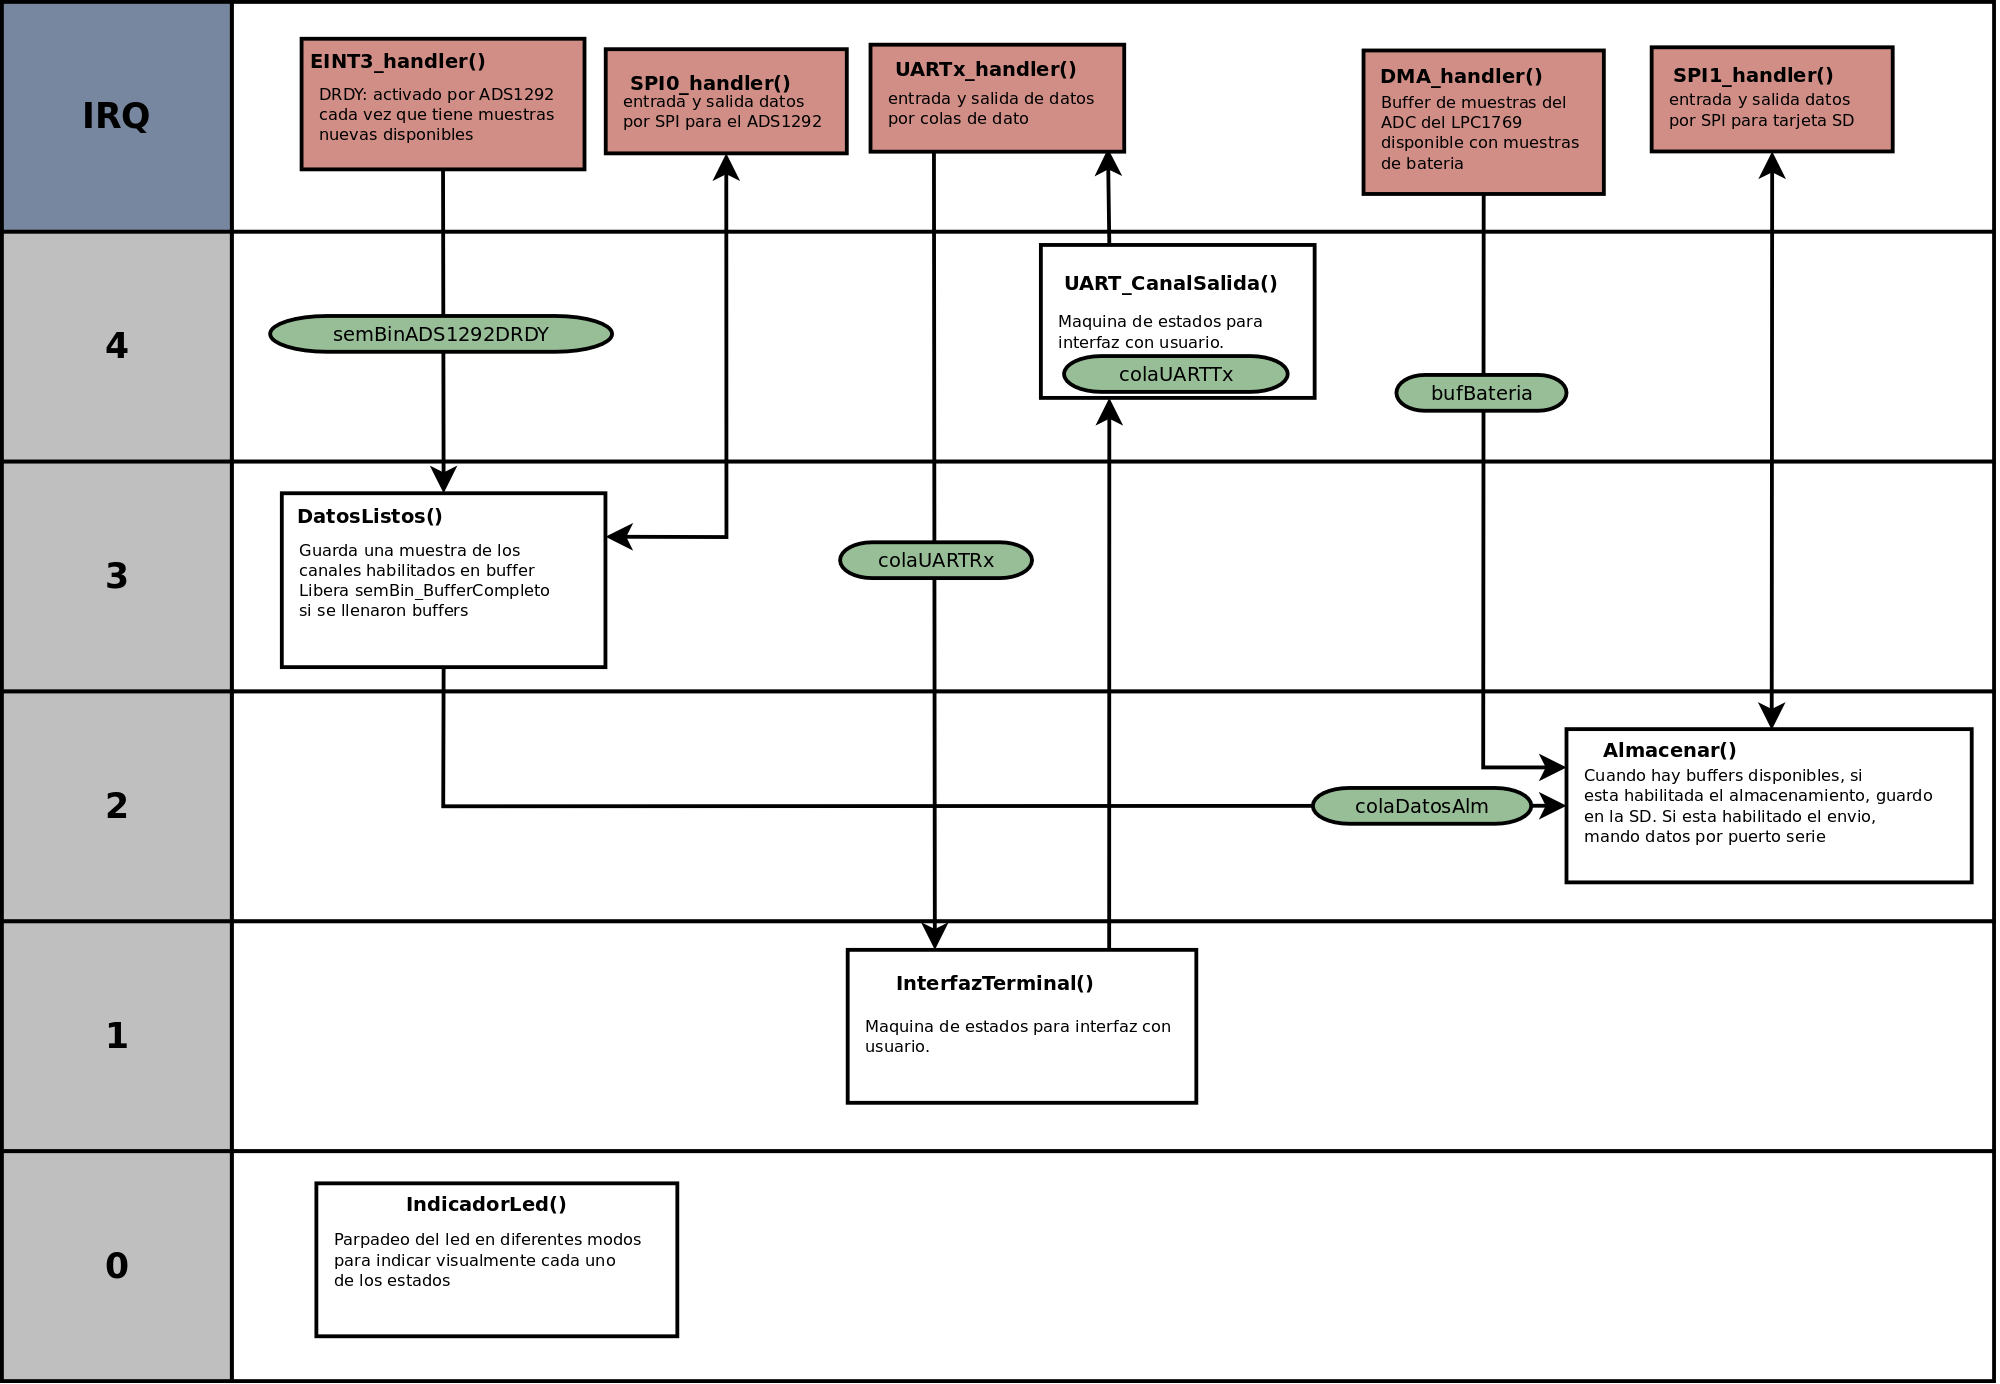
\includegraphics[angle= 90, scale = 0.18]{./Figures/VOP24_tareas_v1_adquirirAlmacenar.png}
\end{adjustbox}


	\item Cuando se conecta el USB a una PC, se activa el handler de la interrupción USB\_Handler y se instala una tarea “InterfazPC()” que espera a que el equipo esté en modo inactivo para luego permitir ver el contenido de la tarjeta de memoria desde la PC como un medio de almacenamiento extraíble. Todas las demás tareas se bloquean mientras el equipo se comunique con la PC: no se puede conectar mediante Bluetooth ni usar ninguna de las funcionalidades anteriores hasta que se desconecte el USB.
	
En este modo el led permanece oscilando para indicar carga y se habilita la carga de la batería. Una vez finalizada la carga, el led queda prendido permanentemente hasta desconectar el USB.

\begin{adjustbox}{center,caption={Diagrama de tareas en modo conexión USB},label={fig:VOP24_tareas_v1_USB},nofloat=figure,vspace=\bigskipamount}
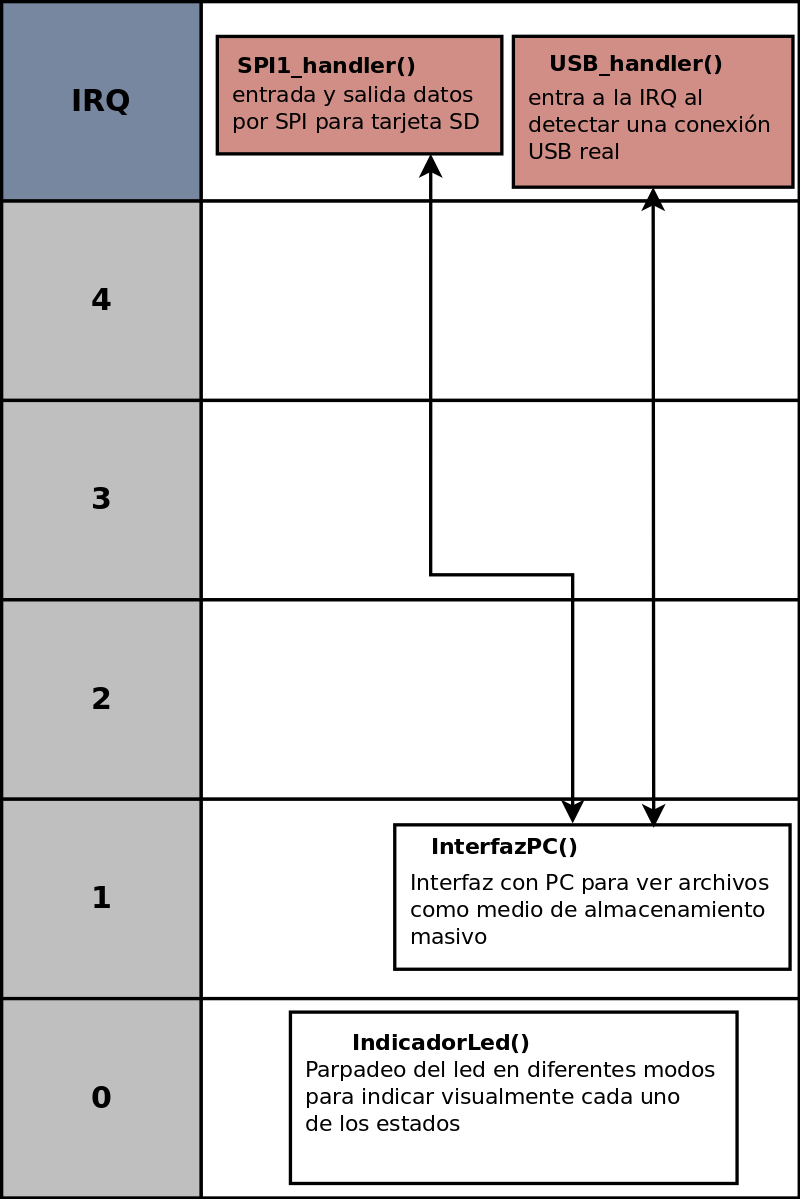
\includegraphics[angle= 0, scale = 0.20]{./Figures/VOP24_tareas_v1_USB.png}
\end{adjustbox}

	\item Durante el modo “configuracion” interviene solamente la comunicación a través de la UART para el caso de modificar hora y fecha. Al momento de calibrar, es necesario activar la medición con el ADS1292, pero en este caso, el buffer adquirido se promedia para obtener solo una muestra como salida. La comunicación con la tarea “DatosListos()” que toma las muestras en el buffer se hace a través de la cola de datos “colaDatosEnv”.

La medición de batería solamente se calibra al momento de grabar el código en la flash, no se ofrece calibración por menú.

\begin{adjustbox}{center,caption={Diagrama de tareas en modo configuración},label={fig:VOP24_tareas_v1_configuracion},nofloat=figure,vspace=\bigskipamount}
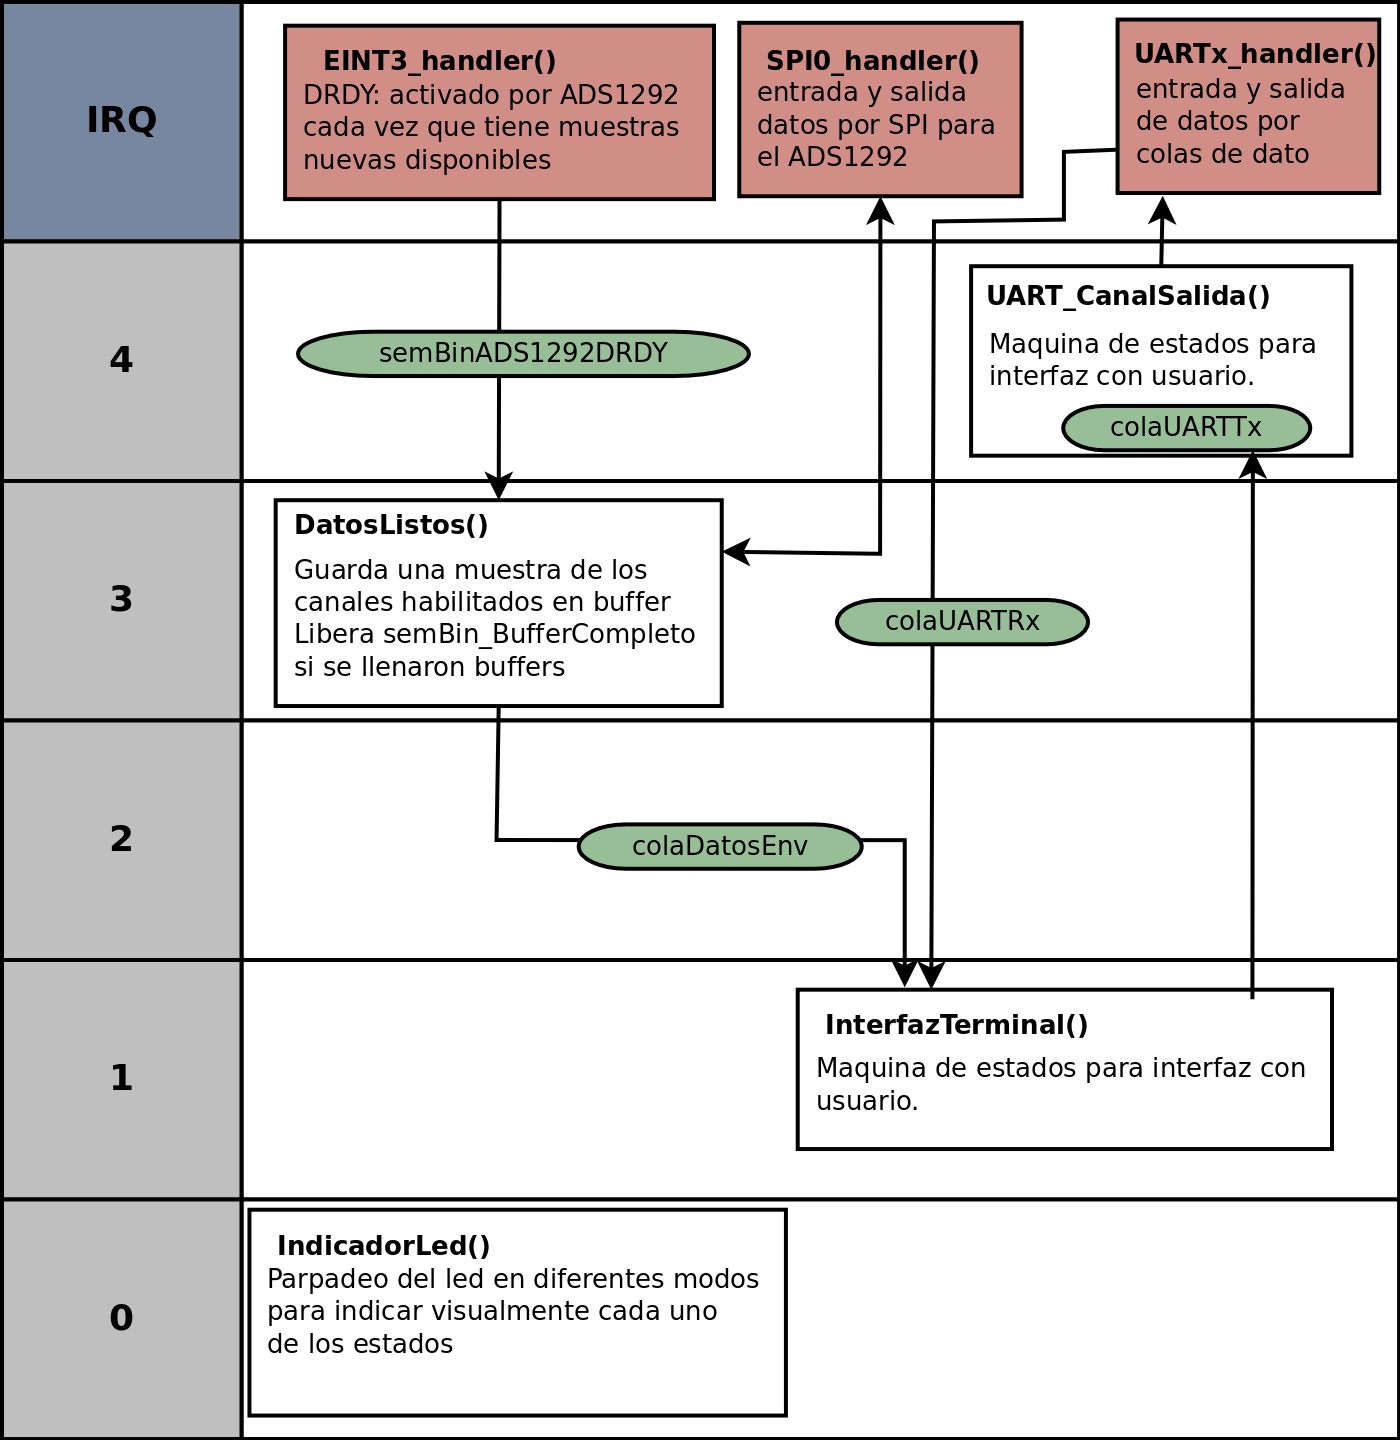
\includegraphics[angle= 90, scale = 0.18]{./Figures/VOP24_tareas_v1_configuracion.png}
\end{adjustbox}

\end{itemize}

\textbf{Diseño de máquinas de estado}

La tarea InterfazTerminal mencionada anteriormente es la encargada de establecer comunicación con el usuario. Se modela como máquina de estados. En la figura \ref{fig:VOP_mde_v1} solamente el flujo posible del programa, no se muestran en el gráfico los comandos específicos que se envían, .


\begin{figure}[!htbp]
	\centering
	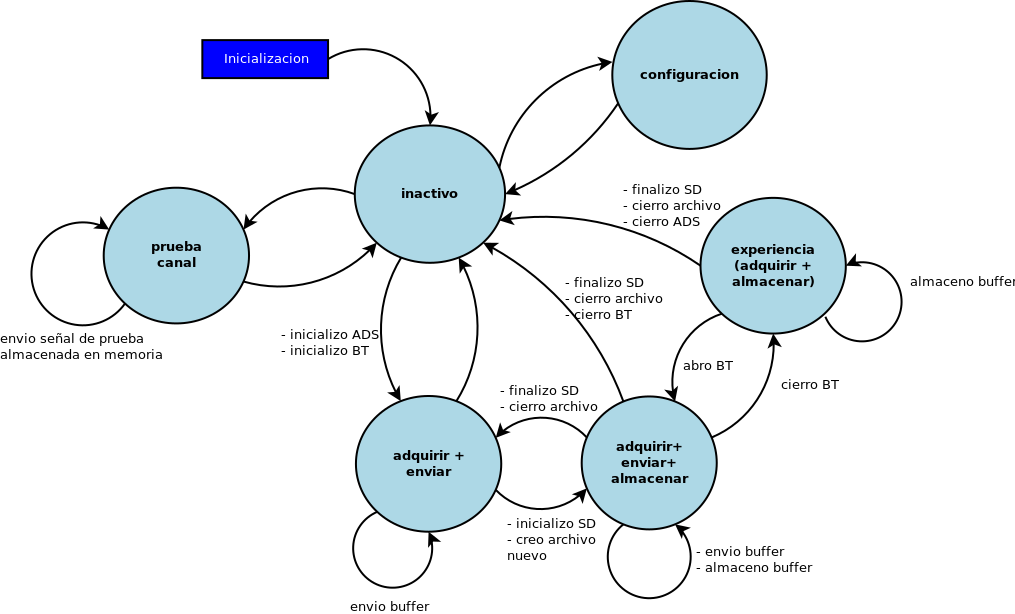
\includegraphics[width=\textwidth]{./Figures/VOP_mde_v1.png}
	\caption{Máquina de estados de tarea de interfaz de usuario}
	\label{fig:VOP_mde_v1}
\end{figure}


El estado de configuración se trata de un estado compuesto en el cual se puede modificar todos los parámetros de adquisición como frecuencia de muestreo, canales habilitados y ganancia PGA. También se  puede cambiar la configuración de fecha y hora y realizar la calibración de un canal. Se modela igualmente como máquina de estados, de acuerdo al diagrama de la figura \ref{fig:VOP24_configuracion_v1}.

\begin{figure}[!htbp]
	\centering
	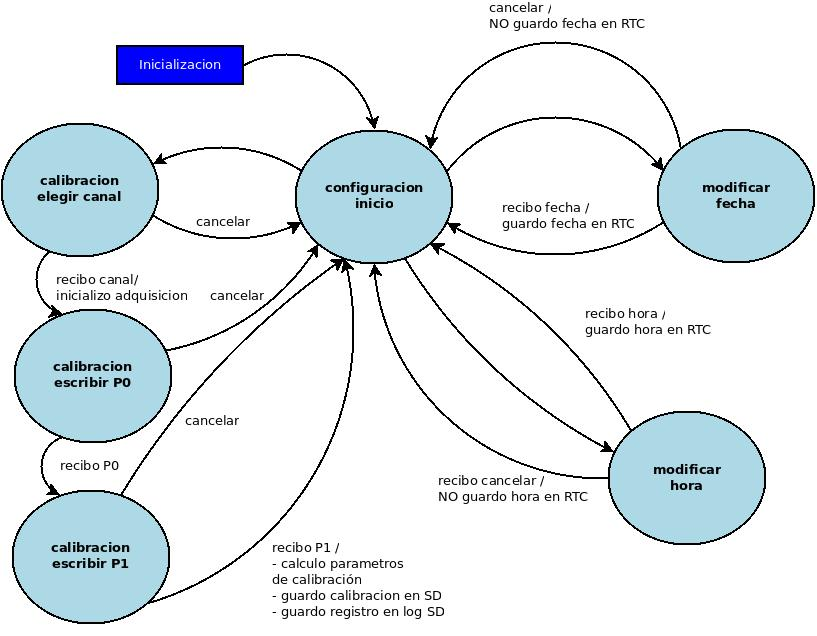
\includegraphics[width=\textwidth]{./Figures/VOP24_configuracion_v1.jpeg}
	\caption{Máquina de estados de configuración de usuario}
	\label{fig:VOP24_configuracion_v1}
\end{figure}

%----------------------------------------------------------------------------------------
%	SECTION 1
%----------------------------------------------------------------------------------------
\section{Análisis del software}
 
En esta sección se resaltan los problemas encontrados, los criterios utilizados y la justificación de las decisiones que se hayan tomado.

Se puede agregar código o pseudocódigo dentro de un entorno lstlisting con el siguiente código:

\begin{verbatim}
\begin{lstlisting] [caption= "un epígrafe descriptivo"]

	las líneas de código irían aquí...
	
\end{lstlisting}
\end{verbatim}

A modo de ejemplo:

\begin{lstlisting}[caption=Pseudocódigo del lazo principal de control.]  % Start your code-block

#define MAX_SENSOR_NUMBER 3
#define MAX_ALARM_NUMBER  6
#define MAX_ACTUATOR_NUMBER 6

uint32_t sensorValue[MAX_SENSOR_NUMBER];		
FunctionalState alarmControl[MAX_ALARM_NUMBER];	//ENABLE or DISABLE
state_t alarmState[MAX_ALARM_NUMBER];						//ON or OFF
state_t actuatorState[MAX_ACTUATOR_NUMBER];			//ON or OFF

void vControl() {

	initGlobalVariables();
	
	period = 500 ms;
		
	while(1) {

		ticks = xTaskGetTickCount();
		
		updateSensors();
		
		updateAlarms();
		
		controlActuators();
		
		vTaskDelayUntil(&ticks, period);
	}
}
\end{lstlisting}



